\documentclass[border=4pt]{standalone}
\usepackage{tikz}
\usetikzlibrary{arrows.meta,positioning,shapes.geometric}
\tikzset{
  process/.style={draw,rounded corners=2pt,minimum width=23mm,minimum height=9mm,align=center},
  decision/.style={diamond,draw,aspect=2,inner sep=1.2pt,align=center}
}
\begin{document}
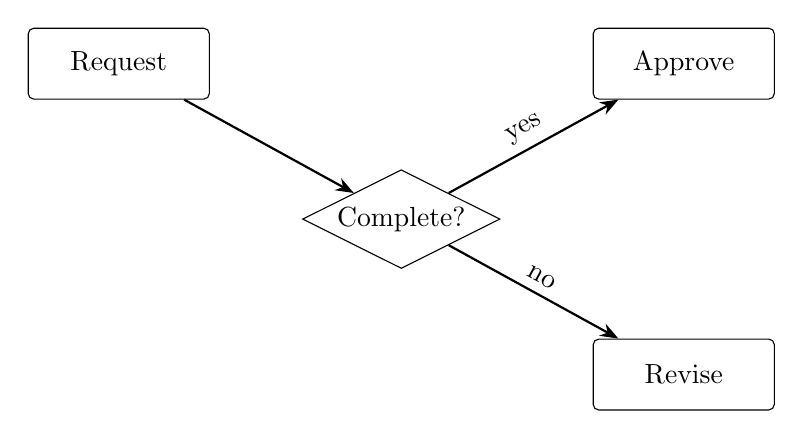
\begin{tikzpicture}[node distance=12mm and 18mm,>=Stealth]
  \node[process] (request) {Request};
  \node[decision,below right=of request] (complete) {Complete?};
  \node[process,above right=of complete] (approve) {Approve};
  \node[process,below right=of complete] (revise) {Revise};
  \draw[->,thick] (request) -- (complete);
  \draw[->,thick] (complete) -- node[above,sloped] {yes} (approve);
  \draw[->,thick] (complete) -- node[above,sloped] {no} (revise);
\end{tikzpicture}
\end{document}
